% Requires: booktabs, siunitx, pgfplots (compat=1.18)
% If you do not use siunitx, replace \SI{0.5}{\metre} with 0.5 m etc.
% All numbers: python3 scripts/analyse_privacy_switch.py study/privacy_switch_study2.csv

\section{Privacy-Switch Reliability}
\label{sec:privacy-switch}

\subsection{Method}
\label{sec:ps-method}

The second study examined whether the assistant moves a confidential spoken
reply to the chat when another person enters the room, whether it refrains
from doing so when someone only passes the door or looks in, and whether it
returns to speech once the visitor has left. A single mover performed four
scripted behaviours at the room's door (Table~\ref{tab:ps-outcomes}): a direct
entry at normal walking pace (script~A, 30 trials), a fast entry at jogging
pace (F, 25), a pass close to the open door without stepping into the doorway
(B, 20), and a peek, in which the mover stopped in the doorway for about
\SI{3}{\second} without entering (D, 18). The test harness presented the
$N = 93$ trials in randomised order. In the entry scripts the mover stayed
inside for \SI{15}{\second} after the switch and then left on a cue from the
harness.

Presence was sensed with an HLK-LD2450 \SI{24}{\giga\hertz} radar module, which
reports up to three targets per frame with position and radial velocity. A
Seeed XIAO ESP32-S3 read the module and relayed each frame over ESP-NOW to a
second XIAO connected to the Raspberry~Pi by USB, where frames arrived at
\SI{10}{\hertz}. Two rectangular zones were defined in the sensor's coordinate
frame, with $x$ lateral and $y$ the distance along the sensor's axis: a room
zone covering the area in which the assistant can be overheard ($x$ from
\SIrange{-1.63}{1.53}{\metre}, $y$ from \SIrange{0.11}{3.79}{\metre}), and a
door zone over the doorway directly beyond it ($x$ from
\SIrange{-1.63}{-0.40}{\metre}, $y$ from \SIrange{3.80}{4.93}{\metre}).

Because the module's three output slots do not preserve a person's identity,
targets were assigned to tracks by greedy nearest-neighbour matching (at most
\SI{0.8}{\metre} between frames; a track ends after \SI{1}{\second} unseen).
Entries and exits were decided at the door zone only. A track passing from the
door zone to at least \SI{100}{\milli\metre} inside the room zone was an entry.
So was a new track first acquired inside the room within \SI{0.8}{\metre} of
the door zone while approaching the sensor at
\SI{150}{\milli\metre\per\second} or more, which covers people who cross the
door zone faster than the module acquires them. A track passing from the room
zone into the door zone and then lost for more than \SI{1}{\second}, or
outside both zones for \SI{1}{\second}, was an exit, as was a new track
acquired in the door zone while receding at \SI{150}{\milli\metre\per\second}
or more. A track that appeared in the door zone and vanished without entering
was a peek. Movement anywhere else could produce neither an entry nor an exit.

With privacy protection enabled (the default), the assistant reacted in three
steps. While it was speaking, anyone in the door zone lowered the voice to a
gain of 0.35 (\SI{-9.1}{\dB}), and normal volume returned \SI{1.5}{\second}
after the door zone was clear. An entry switched the output to the chat:
playback was terminated and the rest of the reply was delivered as text. Once
the last visitor had left, the output returned to speech.

The reply was a ten-sentence confidential message about an overdue payment, a
blood-test result and a rent increase. It was synthesised live by the
assistant's text-to-speech service (ElevenLabs) and played through its
loudspeaker; playback began a median \SI{0.24}{\second} after the harness
requested it. Because the gain is applied before the audio is handed to the
output device, a change in volume becomes audible only once the audio already
queued downstream has played. At the output rate of \SI{16}{\kilo\hertz}, the
configured buffers (a \SI{32}{\milli\second} processing block, a
\SI{128}{\milli\second} pipe and a \SI{150}{\milli\second} ALSA buffer) bound
this delay at about \SI{0.31}{\second}.

Each trial began once the harness had observed the idle state for
\SI{2}{\second}: no visitor counted, nobody in the door zone, normal volume and
speech output. The harness then registered a spoken conversation turn, so that
a conversation partner counted as present, and started the reply. The mover
began the scripted behaviour from a start mark in the corridor as soon as
playback had started. Ground truth was given by the script; after each peek,
the mover additionally confirmed not having stepped into the room.

The harness logged every radar frame and every event of the production
decision logic, timestamped on the Pi. An entry counted as a true positive
when the output switched to the chat within \SI{20}{\second}; a pass or peek
counted as a false positive when it switched at any time within its
\SI{15}{\second} observation window. For peeks, the voice was required to be
lowered without a switch; for passes, it was specified in advance that neither
the volume nor the output should change. The return to speech was classified
from the event log as correct when it occurred after the cue to leave,
premature when it occurred before, and missed when it did not occur within
\SI{60}{\second} of the cue. Moments that the software does not log, such as
the mover crossing the room-zone edge, were estimated from the recorded frames
by linear interpolation between consecutive frames. They are therefore resolved
to about \SI{0.1}{\second} and exclude the module's own measurement latency.
Proportions are reported with exact Clopper--Pearson 95\,\% confidence
intervals (CI), durations as median and interquartile range (IQR).

The target set in the study plan was a miss rate below \SI{5}{\percent},
judged by the upper confidence bound. With 55 entry trials this target could
not have been demonstrated even without a single miss: the upper bound for 0 of
55 is \SI{6.5}{\percent}, and at least 72 consecutive detected entries would
have been needed. The miss rate is therefore reported with its interval rather
than as a pass or fail.

\begin{table}[htbp]
  \centering
  \caption{Outcome per scripted behaviour. \emph{Lowered} counts trials in
  which the voice was lowered at any point. Entries pass through the door zone
  and are expected to be lowered before they switch; one missed fast entry was
  lowered without switching.}
  \label{tab:ps-outcomes}
  \begin{tabular}{llrlrr}
    \toprule
    Script & Behaviour & $n$ & Expected & Switched & Lowered \\
    \midrule
    A & Direct entry, normal pace   & 30 & switch      & 30 & 30 \\
    F & Fast entry                  & 25 & switch      & 23 & 24 \\
    D & Peek, stop in the doorway   & 18 & lower only  &  0 & 18 \\
    B & Pass close to the open door & 20 & no reaction &  0 &  9 \\
    \bottomrule
  \end{tabular}
\end{table}

\subsection{Switch decisions}
\label{sec:ps-switch}

The assistant switched to the chat in 53 of 55 entries (\SI{96.4}{\percent};
CI \SIrange{87.5}{99.6}{\percent}) and in none of the 38 passes and peeks
(CI \SIrange{0}{9.3}{\percent}). All 30 entries at normal pace were detected.
Both misses occurred in fast entries, of which 23 of 25 were detected
(\SI{92.0}{\percent}; CI \SIrange{74.0}{99.0}{\percent}). The observed miss
rate of \SI{3.6}{\percent} lies below the \SI{5}{\percent} target, but its
upper bound of \SI{12.5}{\percent} does not, so the data remain compatible with
a miss rate well above the target. Of the 53 detected entries, 52 were decided
at the door zone. In the remaining one, the mover's track was lost in the door
zone and re-acquired \SI{0.27}{\metre} inside the room while approaching at
\SI{0.96}{\metre\per\second}, so the entry was decided by the near-door rule.

Both misses occurred when the radar failed to follow the fast-moving mover
through the door zone. In one (trial~19), the mover was first reported only
when already inside the room, having crossed the \SI{1.12}{\metre}-deep door
zone unseen. The first radial velocity reported for the new track,
\SI{-80}{\milli\metre\per\second}, did not meet the near-door rule's
\SI{150}{\milli\metre\per\second} condition, although the next frame, taken
\SI{0.1}{\second} later, reported \SI{-1280}{\milli\metre\per\second}. In the
other (trial~37), the mover was detected in the door zone and the voice was
lowered, but the track was then taken over by a reflection that moved out of
both zones with zero radial velocity, while the mover was re-acquired as a new
target \SI{0.96}{\metre} from the door zone, beyond the near-door radius. In
both, the reply went on playing with the visitor in the room: at full volume in
the first, and lowered in the second, where the reflection kept returning into
the door zone. Both failures arise from the few frames a fast entrant spends
in the door zone. For fast entries, the voice was lowered for a median of only
\SI{0.9}{\second} before the switch (Table~\ref{tab:ps-timing}), which
corresponds to about nine frames.

\subsection{Timing of the switch}
\label{sec:ps-timing}

The radar first reported the entrant outside both zones, in the corridor beyond
or beside the doorway, in 39 of the 53 detected entries (median distance from
the sensor \SI{5.09}{\metre}), inside the door zone in 13, and inside the room
in one. Every detected entry lowered the voice before it switched, a median
\SI{1.2}{\second} before the switch (Table~\ref{tab:ps-timing}), so the part of
the reply that played while the entrant crossed the doorway was already
attenuated.

The switch followed the radar-estimated crossing of the room-zone edge by a
median \SI{0.16}{\second} (IQR \SIrange{0.10}{0.18}{\second}, maximum
\SI{0.32}{\second}). This interval is dominated by the \SI{100}{\milli\metre}
entry margin and the \SI{0.1}{\second} frame interval: the software took a
median \SI{0.58}{\milli\second} from the entry event to the switch and a
further \SI{0.35}{\milli\second} to terminate playback. It does not include
the time the module needs to measure and report a position, which cannot be
observed in the logged data.

\begin{table}[htbp]
  \centering
  \small
  \caption{Timing of the 53 detected entries, median [IQR]. Intervals derived
  from radar frames are resolved to the \SI{0.1}{\second} frame interval. The
  room-edge crossing is interpolated between frames and is undefined for the
  entry decided by the near-door rule.}
  \label{tab:ps-timing}
  \begin{tabular}{lccc}
    \toprule
    & Direct entry (A) & Fast entry (F) & All \\
    \midrule
    Ground speed at entry (\si{\metre\per\second})
      & 0.90 [0.82, 1.00] & 1.37 [1.20, 1.44] & 1.02 [0.88, 1.38] \\
    First detection $\to$ switch (\si{\second})
      & 1.95 [1.50, 2.20] & 1.20 [0.90, 1.25] & 1.30 [1.10, 2.00] \\
    Voice lowered $\to$ switch (\si{\second})
      & 1.40 [1.30, 1.50] & 0.90 [0.80, 1.00] & 1.20 [0.90, 1.40] \\
    Room-edge crossing $\to$ switch (\si{\second})
      & 0.17 [0.12, 0.23] & 0.14 [0.09, 0.16] & 0.16 [0.10, 0.18] \\
    \addlinespace
    Entry event $\to$ switch (\si{\milli\second})
      & & & 0.58 [0.45, 0.62] \\
    Switch $\to$ playback terminated (\si{\milli\second})
      & & & 0.35 [0.33, 0.37] \\
    \bottomrule
  \end{tabular}
\end{table}

\subsection{Lowered voice at the door}
\label{sec:ps-door}

Every peek lowered the voice, and none switched the output (18 of 18;
CI \SIrange{81.5}{100}{\percent}). The voice stayed lowered for a median
\SI{8.6}{\second} (IQR \SIrange{8.2}{9.2}{\second}): the time the mover was
registered in the door zone, including approach and retreat (median
\SI{7.0}{\second}), plus the \SI{1.5}{\second} hold. The software changed the
gain a median \SI{0.49}{\milli\second} after the door event, to which the
audio buffering adds up to about \SI{0.31}{\second}.

Passes did not meet the criterion specified in advance. None switched the
output, but 9 of 20 lowered the voice (\SI{45}{\percent}; CI
\SIrange{23.1}{68.5}{\percent}). The radar reported the mover in all 20 passes,
and Figure~\ref{fig:ps-door-depth} shows why the outcome varied: a close pass
ran along the outer edge of the door zone. Passes that lowered the voice
reached a median \SI{0.07}{\metre} past that edge (at most
\SI{0.26}{\metre}); those that did not came within a median \SI{0.08}{\metre}
of it. Whether a pass lowered the voice was therefore decided by a few
centimetres of reported position. Peeks, in contrast, reached
\SIrange{0.21}{0.52}{\metre} into the door zone. Moving its outer edge inwards
by \SI{0.15}{\metre} would have separated passes from peeks in all but one
trial. Because this margin was derived after the fact from the same data, it
is a starting point rather than a validated setting.

A lowered voice for someone close enough to the doorway to be seen is in the
spirit of the graded response, since anyone within earshot at the door hears
less. It was nevertheless not the behaviour specified, and is reported as a
deviation. Its cost was small: the reply continued without interruption and
returned to normal volume a median \SI{5.1}{\second} after it had been lowered.

\begin{figure}[htbp]
  \centering
  \definecolor{passc}{HTML}{2A78D6}
  \definecolor{peekc}{HTML}{EB6834}
  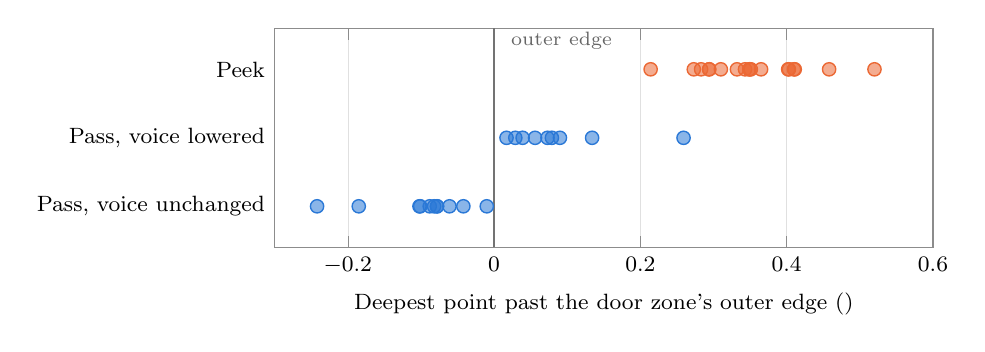
\begin{tikzpicture}
    \begin{axis}[
      width=0.82\textwidth, height=0.36\textwidth,
      xmin=-0.3, xmax=0.6, ymin=0.4, ymax=3.6,
      xlabel={Deepest point past the door zone's outer edge (\si{\metre})},
      ytick={1,2,3},
      yticklabels={{Pass, voice unchanged},{Pass, voice lowered},{Peek}},
      tick label style={font=\footnotesize},
      label style={font=\footnotesize},
      xmajorgrids, grid style={line width=0.2pt, draw=black!12},
      axis line style={draw=black!45}, tick style={draw=black!45},
      ytick style={draw=none},
    ]
      \addplot[black!55, line width=0.6pt, forget plot] coordinates {(0,0.4) (0,3.6)};
      \node[font=\scriptsize, black!60, anchor=south west] at (axis cs:0.01,3.15) {outer edge};
      \addplot[only marks, mark=*, mark size=2.4pt,
               mark options={fill=passc, fill opacity=0.55, draw=passc, line width=0.5pt}]
        coordinates {(-0.242,1) (-0.185,1) (-0.082,1) (-0.102,1) (-0.078,1) (-0.088,1)
                     (-0.078,1) (-0.061,1) (-0.042,1) (-0.010,1) (-0.101,1)};
      \addplot[only marks, mark=*, mark size=2.4pt,
               mark options={fill=passc, fill opacity=0.55, draw=passc, line width=0.5pt}]
        coordinates {(0.259,2) (0.017,2) (0.056,2) (0.134,2) (0.039,2) (0.079,2)
                     (0.029,2) (0.073,2) (0.090,2)};
      \addplot[only marks, mark=*, mark size=2.4pt,
               mark options={fill=peekc, fill opacity=0.55, draw=peekc, line width=0.5pt}]
        coordinates {(0.402,3) (0.411,3) (0.351,3) (0.343,3) (0.410,3) (0.310,3)
                     (0.273,3) (0.294,3) (0.283,3) (0.403,3) (0.294,3) (0.332,3)
                     (0.365,3) (0.458,3) (0.214,3) (0.349,3) (0.349,3) (0.520,3)};
    \end{axis}
  \end{tikzpicture}
  \caption{How far each pass and peek reached into the door zone, measured from
  its outer edge on the corridor side. Negative values give the closest
  approach of the passes that stayed outside. Passes ran along the edge, within
  \SI{0.26}{\metre} of it on either side; peeks reached
  \SIrange{0.21}{0.52}{\metre} into the zone. One point per trial.}
  \label{fig:ps-door-depth}
\end{figure}

\subsection{Return to speech}
\label{sec:ps-return}

Table~\ref{tab:ps-return} classifies what happened after the 53 detected
entries. In 44, the voice returned correctly after the mover had left, a median
\SI{2.35}{\second} (IQR \SIrange{2.16}{2.56}{\second}) after the mover's track
crossed from the room back into the door zone. This comprises the walk through
the door zone and the \SI{1}{\second} for which a track must be lost or outside
before an exit is confirmed. In one entry (trial~16) the voice never returned:
on the way out, the mover's reported path passed the doorway
\SIrange{0.34}{0.53}{\metre} to the side of the door zone, which the logic by
design does not accept as an exit. This failure is safe, since the output
simply remains in the chat.

The remaining eight entries (\SI{15.1}{\percent}; CI
\SIrange{6.7}{27.6}{\percent}) returned to speech prematurely,
\SIrange{2.2}{9.1}{\second} after the switch (median \SI{3.7}{\second}), while
the mover was still inside, a median \SI{11.4}{\second} before the cue to
leave. In seven of them the mover was being tracked inside the room at that
very moment; in the eighth, the mover was re-acquired inside
\SI{0.5}{\second} later. This is the one failure observed in the study that
works against privacy. The interrupted reply was not resumed aloud, but from
that moment on any further reply would have been spoken with the visitor
present.

The harness's own summary, which considered only returns after the cue,
reported 45 of 53 returns. It counted seven premature returns and the missed
one as failures to return, and one premature return as correct because the
mover later re-entered and left again. The classification here is derived from
the complete event log.

\begin{table}[htbp]
  \centering
  \caption{Return to speech after the 53 detected entries, classified from the
  event log.}
  \label{tab:ps-return}
  \begin{tabular}{lrrl}
    \toprule
    Outcome & $n$ & \% [95\,\% CI] & Consequence \\
    \midrule
    Correct, after the mover left            & 44 & 83.0 [70.2, 91.9] & --- \\
    Premature, with the mover inside         &  8 & 15.1 [6.7, 27.6]  & speech with a visitor present \\
    Missed, no return within \SI{60}{\second} &  1 & 1.9 [0.0, 10.1]   & reply stays in the chat \\
    \bottomrule
  \end{tabular}
\end{table}

All eight premature returns share one mechanism, shown for one trial in
Figure~\ref{fig:ps-phantom}. Shortly after the entrant stopped inside the room,
the module's report for that person moved back towards the doorway, while the
mover reappeared as a new target further inside. Because the drifting report
moved only a short distance per frame, the nearest-neighbour association kept
the entrant's identity on it. It then crossed from the room into the door zone
and vanished, exactly as a departing visitor would.

\begin{figure}[htbp]
  \centering
  \definecolor{entc}{HTML}{EB6834}
  \definecolor{movc}{HTML}{2A78D6}
  \begin{tikzpicture}
    \begin{axis}[
      axis equal image,
      width=0.5\textwidth, height=0.8\textwidth,
      xmin=-2.6, xmax=0.6, ymin=1.9, ymax=5.8,
      xtick={-2,-1,0}, ytick={2,3,4,5},
      xlabel={$x$ (\si{\metre})}, ylabel={$y$ (\si{\metre})},
      tick label style={font=\footnotesize},
      label style={font=\footnotesize},
      axis line style={draw=black!45}, tick style={draw=black!45},
      legend style={at={(1.04,0)}, anchor=south west, font=\scriptsize,
                    draw=none, cells={anchor=west}},
    ]
      \draw[black!40, fill=black!4] (axis cs:-1.630,0.107) rectangle (axis cs:1.531,3.794);
      \draw[black!40, dashed, fill=black!10] (axis cs:-1.630,3.804) rectangle (axis cs:-0.399,4.926);
      \node[font=\scriptsize, black!60, anchor=north east] at (axis cs:0.55,3.74) {room zone};
      \node[font=\scriptsize, black!60, anchor=west] at (axis cs:-0.36,4.40) {door zone};
      \addplot[entc, line width=1pt, mark=*, mark size=0.9pt]
        coordinates {(-1.53,4.78) (-1.51,4.66) (-1.48,4.59) (-1.43,4.53) (-1.32,4.44)
                     (-1.18,4.35) (-1.06,4.25) (-0.97,4.18) (-0.97,3.97) (-1.04,3.84)
                     (-1.09,3.70) (-1.16,3.56) (-1.22,3.45) (-1.22,3.55) (-1.22,3.66)
                     (-1.22,3.69) (-1.22,3.72) (-1.23,3.74) (-1.25,3.76) (-1.32,3.81)
                     (-1.39,3.85) (-1.47,3.87) (-1.54,3.88) (-1.61,3.90) (-1.76,3.91)
                     (-1.83,3.92) (-1.89,3.92) (-1.93,3.93) (-1.96,3.93) (-1.98,3.93)
                     (-2.00,3.93) (-2.02,3.94) (-2.06,3.94) (-2.08,3.94) (-2.10,3.95)
                     (-2.11,3.95)};
      \addlegendentry{entrant's track, \SIrange{3.4}{6.9}{\second}}
      \addplot[movc, line width=0.8pt, mark=*, mark size=0.6pt]
        coordinates {(-0.64,2.52) (-0.46,2.40) (-0.46,2.37) (-0.44,2.40) (-0.58,2.51)
                     (-0.75,2.53) (-0.81,2.57) (-0.88,2.56) (-0.86,2.58) (-0.80,2.60)
                     (-0.78,2.60) (-0.75,2.61) (-0.69,2.62) (-0.65,2.64) (-0.63,2.66)
                     (-0.61,2.68) (-0.60,2.69) (-0.57,2.69) (-0.55,2.68) (-0.54,2.67)
                     (-0.57,2.67) (-0.56,2.67) (-0.57,2.67) (-0.60,2.67) (-0.56,2.69)
                     (-0.57,2.68) (-0.56,2.66) (-0.56,2.65) (-0.54,2.62) (-0.54,2.61)
                     (-0.55,2.58) (-0.50,2.44) (-0.53,2.34) (-0.62,2.25) (-0.64,2.21)
                     (-0.62,2.21) (-0.64,2.21) (-0.65,2.22) (-0.63,2.24) (-0.67,2.25)
                     (-0.73,2.28) (-0.68,2.34) (-0.65,2.40) (-0.66,2.42) (-0.65,2.44)
                     (-0.64,2.45) (-0.61,2.45) (-0.64,2.44) (-0.67,2.43) (-0.65,2.44)
                     (-0.63,2.44) (-0.61,2.46) (-0.58,2.48) (-0.55,2.54) (-0.58,2.58)
                     (-0.63,2.63) (-0.68,2.75) (-0.71,2.94) (-0.76,3.07) (-0.83,3.20)
                     (-0.92,3.31) (-1.04,3.52) (-1.18,3.64) (-1.35,3.76) (-1.45,3.90)
                     (-1.43,4.17) (-1.32,4.37) (-1.19,4.55) (-1.14,4.74) (-1.05,5.02)
                     (-1.16,5.18) (-1.22,5.29) (-1.21,5.38) (-1.26,5.48) (-1.28,5.50)
                     (-1.29,5.52) (-1.30,5.54) (-1.31,5.56) (-1.32,5.56)};
      \addlegendentry{mover re-acquired, \SIrange{5.6}{26.5}{\second}}
      \addplot[only marks, mark=*, mark size=1.6pt, black, forget plot]
        coordinates {(-1.53,4.78) (-1.16,3.56) (-2.11,3.95)};
      \addplot[only marks, mark=o, mark size=2.6pt, black, line width=0.8pt, forget plot]
        coordinates {(-0.63,2.52)};
      \node[circle, draw=black!60, fill=white, inner sep=0.8pt, font=\scriptsize] at (axis cs:-1.80,4.90) {1};
      \node[circle, draw=black!60, fill=white, inner sep=0.8pt, font=\scriptsize] at (axis cs:-0.74,3.60) {2};
      \node[circle, draw=black!60, fill=white, inner sep=0.8pt, font=\scriptsize] at (axis cs:-2.24,3.62) {3};
      \node[circle, draw=black!60, fill=white, inner sep=0.8pt, font=\scriptsize] at (axis cs:-1.00,2.46) {4};
    \end{axis}
  \end{tikzpicture}
  \caption{A premature return to speech (trial~41, fast entry), in the sensor's
  coordinates; the sensor sits at the origin, below the plotted area, facing
  the door. (1)~The mover is detected in the door zone at \SI{3.4}{\second}
  and the voice is lowered. (2)~At \SI{4.6}{\second} the mover enters and the
  output switches to the chat. The report for the entrant then slides out of
  the room to the left while its radial velocity reads \SIrange{0}{80}{\milli
  \metre\per\second}. (3)~At \SI{6.9}{\second} it is confirmed as an exit and
  the output returns to speech, although the mover is standing inside (4),
  where the radar had re-acquired the mover as a new target at
  \SI{5.6}{\second}. The mover actually leaves at \SI{23}{\second}, along the
  blue path through the door zone.}
  \label{fig:ps-phantom}
\end{figure}

The drifting report was not the mover. Its reported radial velocity was a
median \SI{0}{\milli\metre\per\second} (per-trial medians between
\SI{-80}{} and \SI{80}{\milli\metre\per\second}), whereas the change in its
reported distance from the sensor implied that it was receding at a median
\SI{0.52}{\metre\per\second} (range \SIrange{0.13}{1.84}{\metre\per\second}).
For genuine exits the two measures agreed, with a median
\SI{0.92}{\metre\per\second} reported against \SI{0.98}{\metre\per\second}
derived from position. Whether the spurious target originates from a multipath
reflection or from the module's internal tracking cannot be determined from
the recorded data.

The reported radial velocity also separates the two kinds of exit completely
in this data set. Within \SI{0.5}{\second} of crossing into the door zone,
every genuine exit reached at least \SI{720}{\milli\metre\per\second} (median
\SI{1120}{\milli\metre\per\second}), whereas no premature one exceeded
\SI{160}{\milli\metre\per\second}.

After the study, this observation was turned into a condition in the decision
logic: an exit is accepted only if the track moves away from the sensor at
\SI{0.5}{\metre\per\second} or more at some point on its way out, from
\SI{0.5}{\second} before it reaches the door zone until the exit is confirmed.
The threshold is about half a normal walking pace. Its effect was assessed by
replaying the recorded radar frames of all 93 trials offline through the
production decision logic (Table~\ref{tab:ps-replay}). Replayed through the
logic used in the study, the frames reproduced the observed outcome of every
trial and the time of every return to speech to within \SI{1}{\milli\second},
which confirms that the replay is faithful. With the condition added, entries
and false switches were unchanged, and none of the returns to speech was
premature.

The price is three missed returns instead of one, all of the safe kind, in
which the reply stays in the chat. Two occurred where the mover's reported path
left the room beside the door zone: the one already missed in the study, and
one that had returned correctly only because the phantom happened to vanish
just as the mover walked out. In the third, the mover had been lost inside the
room and re-acquired near the door while moving inwards, which the near-door
rule counted as a second visitor. In the study, the phantom's false exit had
cancelled this error.

The replay shows that the condition turns the observed privacy failures into
safe ones on these trials; it does not show how the condition performs on new
data. Both the condition and its threshold were derived from the same trials,
and no further trials could be run within this work. The replayed outcome was,
however, identical for any threshold between \SI{0.4}{} and
\SI{0.7}{\metre\per\second}, whereas at \SI{0.3}{\metre\per\second} one
premature return remained. A first version that accepted the speed only within
\SI{0.5}{\second} of reaching the door zone missed four returns, because a
phantom waiting in the door zone could absorb the mover's actual exit.

\begin{table}[htbp]
  \centering
  \caption{Outcomes observed in the study and in the offline replay of its
  93 trials, with the decision logic used in the study and with the exit
  condition added afterwards.}
  \label{tab:ps-replay}
  \begin{tabular}{lrrr}
    \toprule
    & Observed & \multicolumn{2}{c}{Replay} \\
    \cmidrule(lr){3-4}
    & & Study logic & With exit condition \\
    \midrule
    Entries detected (of 55)      & 53 & 53 & 53 \\
    False switches (of 38)        &  0 &  0 &  0 \\
    \addlinespace
    Return to speech: correct     & 44 & 44 & 50 \\
    Return to speech: premature   &  8 &  8 &  0 \\
    Return to speech: missed      &  1 &  1 &  3 \\
    \bottomrule
  \end{tabular}
\end{table}

\subsection{Limitations}

\begin{itemize}
  \item All trials were performed by a single mover (the author), who knew the
  system and the protocol, in one room with one door and one sensor placement,
  and the zones were drawn for this geometry. Visitors who hesitate, turn back
  in the doorway or enter side by side were not tested; two people close
  together may be reported as a single target.

  \item The miss-rate target could not be demonstrated by design, and the
  observed interval (\SIrange{0.4}{12.5}{\percent}) remains compatible with a
  miss rate well above it. The same applies to false switches, whose upper
  bound is \SI{9.3}{\percent}.

  \item All times were taken from the Pi's clock and the recorded radar frames.
  The module's own latency and the acoustic onset and offset of the voice were
  not measured independently, and the audible delay of the lowered voice is
  bounded from the buffer configuration rather than measured. The trials were
  video-recorded, and the harness can merge timings read off the video, but
  this was not done for the present analysis.

  \item Whether a gain of 0.35 makes the reply unintelligible at the door was
  not measured. The lowered voice is evaluated here as a reaction, not as a
  protection.

  \item The door-zone margin in Section~\ref{sec:ps-door} and the exit
  condition in Section~\ref{sec:ps-return} were derived after the fact from the
  same trials. The replay confirms the implementation of the exit condition and
  its trade-off on these trials, but not its performance on new data, which
  could not be tested within this work.

  \item The conversation partner was simulated by a registered turn, so the
  logic that decides whether the user has left was not exercised. The harness
  let the operator discard a trial before saving it, intended for procedural
  errors, and discarded attempts were not logged. One pass was recorded with
  an earlier revision of the exit logic, which does not affect a trial in which
  nobody enters.

  \item Although only one person was present, \SI{14.7}{\percent} of the
  frames containing a target reported two or more targets, in 27 of 93 trials.
  Spurious targets caused no false switch, since an entry must pass through
  the door zone, but a spurious target leaving through it produced all eight
  premature returns. With several people in the room, association errors of
  this kind are likely to become more frequent.
\end{itemize}
